
\lettrine[lines=3]{T}{he MC methodology} mainly considers two types of point-based temporal logics (PTLs) as the property specification language---\emph{linear} and \emph{branching}---which differ 
in the underlying model of time.
In linear PTLs, such as $\LTL$~\cite{Pnu77}, each moment in time has a unique possible future:
formulas are interpreted over (infinite) \emph{paths} of a Kripke structure, and thus they refer to a single computation of a system.
In branching PTLs,
such as $\CTL$ and $\CTLStar$~\cite{EH86}, each moment in time may evolve into several possible futures:
formulas are interpreted over \emph{states} of the Kripke structure, hence referring to all the possible system computations.

In the previous chapters we have assumed a \emph{state-based} semantics for $\HS$, which
induces a branching reference both in the future and in the past:
intervals/traces 
are \lq\lq forgetful\rq\rq{} of the history leading to their initial state, and  
the initial (resp., final) state of an interval may feature several predecessors (resp., successors).
A graphical account of the state-based semantics can be found in Figure~\ref{fig:ST}; a detailed explanation will be given in the following.

\begin{figure}[tp]
\centering
\begin{minipage}{0.36\linewidth}
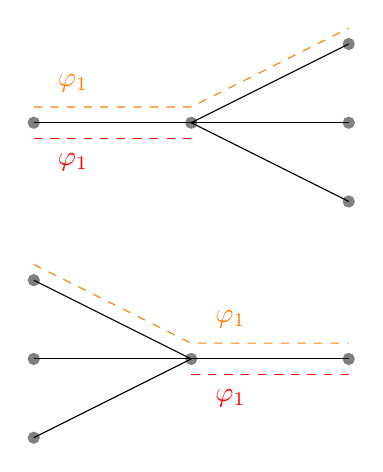
\begin{tikzpicture}
				%				[->,>=stealth',shorten >=1pt,auto,node distance=0,main node/.style={circle,draw}]
				\filldraw [gray] (0,2) circle (2pt)
				(2,2) circle (2pt)
				(4,3) circle (2pt)
				(4,2) circle (2pt)
				(4,1) circle (2pt);
				%
					\filldraw [gray] (4,-1) circle (2pt)
				(2,-1) circle (2pt)
				(0,0) circle (2pt)
				(0,-1) circle (2pt)
				(0,-2) circle (2pt);
				%
				\draw [black]  (0,2) -- (4,2);
				\draw [black]  (0,-1) -- (4,-1);
				%
				\draw [black] (2,2) -- (4,3);
				\draw [black] (2,2) -- (4,1);
				\draw [black] (0,0) -- (2,-1);
				\draw [black] (0,-2) -- (2,-1);
				%
				\draw [dashed, orange] (0,2.2) -> (2,2.2) -> (4,3.2);
				\draw [dashed, red] (0,1.8) -> (2,1.8);
				\draw [dashed, orange] (0,0.2) -> (2,-0.8) -> (4,-0.8);
				\draw [dashed, red] (2,-1.2) -> (4,-1.2);
				
	%		{\tiny
				\node [orange] at (0.5,2.5) {$\varphi_1$};	
				\node [red] at (0.5,1.5) {$\hsBt\varphi_1$};
			\node [orange] at (2.5,-0.5) {$\varphi_1$};	
				\node [red] at (2.5,-1.5) {$\hsEt\varphi_1$};
		%			\node (b0) at (4,-0.5) {$\rho'=\rho(0,i)\cdot \rho^{(j+1)]}$};	
		%			\node (a1) at (1.5,0.2) {$\rho(i)=$};
		%			\node (a2) at (2,0.2) {$\rho(j)$};
		%			\node (a3) at (1.65,0.5) {$Pattern(\rho,i)= Pattern(\rho,j)$};
		%			\node (a4) at (4.6,0.5) {$Pattern(\rho,k) =\{ p \in \Prop : \Ku,\rho^{k]} \models p\}$};
						
	%			}
				
			\end{tikzpicture}
\end{minipage}	
\hfill 	
\begin{minipage}{0.54\linewidth}
			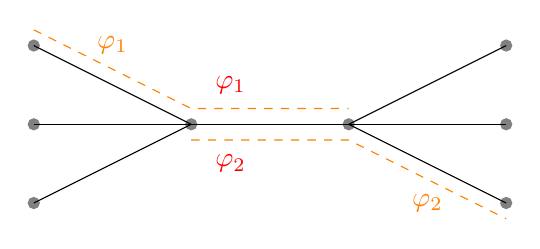
\begin{tikzpicture}
				%				[->,>=stealth',shorten >=1pt,auto,node distance=0,main node/.style={circle,draw}]
				%
					\filldraw [gray] (4,-1) circle (2pt)
				(2,-1) circle (2pt)
				(0,0) circle (2pt)
				(0,-1) circle (2pt)
				(0,-2) circle (2pt)
				(6,0) circle (2pt)
				(6,-1) circle (2pt)
				(6,-2) circle (2pt)	;
				%
				\draw [black]  (0,-1) -- (6,-1);
				%
				\draw [black] (4,-1) -- (6,0);
				\draw [black] (4,-1) -- (6,-2);
					\draw [black] (0,0) -- (2,-1);
				\draw [black] (0,-2) -- (2,-1);
				%
				\draw [dashed, orange] (0,0.2) -> (2,-0.8) -> (4,-0.8);
				\draw [dashed, orange] (2,-1.2) -> (4,-1.2) -> (6,-2.2);
				
	%		{\tiny
				\node [orange] at (1,0) {$\varphi_1$};	
				\node [red] at (2.5,-0.5) {$\hsAt\varphi_1$};
			\node [orange] at (5,-2) {$\varphi_2$};	
				\node [red] at (2.5,-1.5) {$\hsA \varphi_2$};
		%			\node (b0) at (4,-0.5) {$\rho'=\rho(0,i)\cdot \rho^{(j+1)]}$};	
		%			\node (a1) at (1.5,0.2) {$\rho(i)=$};
		%			\node (a2) at (2,0.2) {$\rho(j)$};
		%			\node (a3) at (1.65,0.5) {$Pattern(\rho,i)= Pattern(\rho,j)$};
		%			\node (a4) at (4.6,0.5) {$Pattern(\rho,k) =\{ p \in \Prop : \Ku,\rho^{k]} \models p\}$};
						
	%			}
				
			\end{tikzpicture}
\end{minipage}
%
    \caption{State-based semantic variant $\HS_\stat$: past and future are branching}
    \label{fig:ST}
\end{figure}

However, as we already said, $\HS$ MC has been simultaneously and independently studied also by Lomuscio and Michaliszyn in~\cite{LM13,LM14,lm16}:
there, the considered $\HS$ fragments are interpreted over the unwinding of a Kripke structure (\emph{computation-tree-based} semantics---see Figure~\ref{fig:CT}). %, and interval labeling takes into account only the endpoints of intervals. 
This induces a linear reference in the past (the initial state of an interval may feature only one predecessor), but branching in the future (the final state features several successors). Moreover, the computation history is never forgotten and increases with time.

\begin{figure}[tp]
\centering
\begin{minipage}{0.36\linewidth}
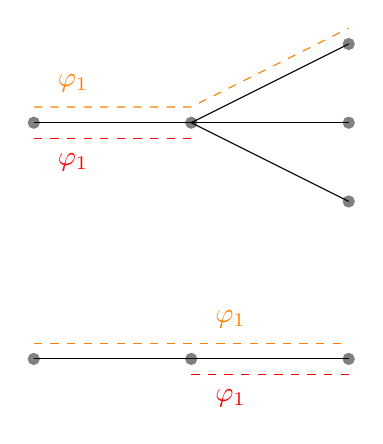
\begin{tikzpicture}
				%				[->,>=stealth',shorten >=1pt,auto,node distance=0,main node/.style={circle,draw}]
				\filldraw [gray] (0,2) circle (2pt)
				(2,2) circle (2pt)
				(4,3) circle (2pt)
				(4,2) circle (2pt)
				(4,1) circle (2pt);
				%
					\filldraw [gray] (4,-1) circle (2pt)
				(2,-1) circle (2pt)
				%(0,0) circle (2pt)
				(0,-1) circle (2pt);
				%(0,-2) circle (2pt);
				%
				\draw [black]  (0,2) -- (4,2);
				\draw [black]  (0,-1) -- (4,-1);
				%
				\draw [black] (2,2) -- (4,3);
				\draw [black] (2,2) -- (4,1);
				%\draw [black] (0,0) -- (2,-1);
				%\draw [black] (0,-2) -- (2,-1);
				%
				\draw [dashed, orange] (0,2.2) -> (2,2.2) -> (4,3.2);
				\draw [dashed, red] (0,1.8) -> (2,1.8);
				\draw [dashed, orange] (0,-0.8) -> (2,-0.8) -> (4,-0.8);
				\draw [dashed, red] (2,-1.2) -> (4,-1.2);
				
	%		{\tiny
				\node [orange] at (0.5,2.5) {$\varphi_1$};	
				\node [red] at (0.5,1.5) {$\hsBt\varphi_1$};
			\node [orange] at (2.5,-0.5) {$\varphi_1$};	
				\node [red] at (2.5,-1.5) {$\hsEt\varphi_1$};
		%			\node (b0) at (4,-0.5) {$\rho'=\rho(0,i)\cdot \rho^{(j+1)]}$};	
		%			\node (a1) at (1.5,0.2) {$\rho(i)=$};
		%			\node (a2) at (2,0.2) {$\rho(j)$};
		%			\node (a3) at (1.65,0.5) {$Pattern(\rho,i)= Pattern(\rho,j)$};
		%			\node (a4) at (4.6,0.5) {$Pattern(\rho,k) =\{ p \in \Prop : \Ku,\rho^{k]} \models p\}$};
						
	%			}
				
			\end{tikzpicture}
\end{minipage}			
\hfill
\begin{minipage}{0.54\linewidth}
			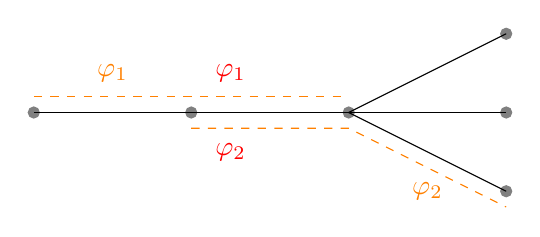
\begin{tikzpicture}
				%				[->,>=stealth',shorten >=1pt,auto,node distance=0,main node/.style={circle,draw}]
				%
					\filldraw [gray] (4,-1) circle (2pt)
				(2,-1) circle (2pt)
				%(0,0) circle (2pt)
				(0,-1) circle (2pt)
				%(0,-2) circle (2pt)
				(6,0) circle (2pt)
				(6,-1) circle (2pt)
				(6,-2) circle (2pt)	;
				%
				\draw [black]  (0,-1) -- (6,-1);
				%
				\draw [black] (4,-1) -- (6,0);
				\draw [black] (4,-1) -- (6,-2);
				% \draw [black] (0,0) -- (2,-1);
				% \draw [black] (0,-2) -- (2,-1);
				%
				\draw [dashed, orange] (0,-0.8) -> (2,-0.8) -> (4,-0.8);
				\draw [dashed, orange] (2,-1.2) -> (4,-1.2) -> (6,-2.2);
				
	%		{\tiny
				\node [orange] at (1,-0.5) {$\varphi_1$};	
				\node [red] at (2.5,-0.5) {$\hsAt\varphi_1$};
			\node [orange] at (5,-2) {$\varphi_2$};	
				\node [red] at (2.5,-1.5) {$\hsA \varphi_2$};
		%			\node (b0) at (4,-0.5) {$\rho'=\rho(0,i)\cdot \rho^{(j+1)]}$};	
		%			\node (a1) at (1.5,0.2) {$\rho(i)=$};
		%			\node (a2) at (2,0.2) {$\rho(j)$};
		%			\node (a3) at (1.65,0.5) {$Pattern(\rho,i)= Pattern(\rho,j)$};
		%			\node (a4) at (4.6,0.5) {$Pattern(\rho,k) =\{ p \in \Prop : \Ku,\rho^{k]} \models p\}$};
						
	%			}
				
			\end{tikzpicture}
\end{minipage}
%
    \caption{Computation-tree-based semantic variant $\HS_\LinearPast$: future is branching, past is linear, finite and cumulative.}
    \label{fig:CT}
\end{figure}

In this chapter, we study the expressiveness of $\HS$, in the context of MC, in comparison with that of the standard PTLs $\LTL$, $\CTL$, and $\CTLStar$. The analysis is carried on \emph{enforcing the homogeneity assumption}.
% 
We prove that $\HS$ endowed with the state-based semantics (hereafter denoted as $\HS_\stat$) is not comparable with $\LTL$, $\CTL$, and $\CTLStar$. On one hand, the result supports the intuition that $\HS_\stat$ gains some expressiveness by the ability of branching in the past. On the other hand, $\HS_\stat$ does not feature the possibility of forcing the verification of a property over an %linear 
infinite path, thus implying that the formalisms are not comparable. With the aim of having a more ``effective'' comparison base, we consider two additional semantic variants of $\HS$, 
%besides the state-based one $\HS_\stat$, 
namely, the \emph{computation-tree-based semantic variant} (denoted as $\HS_\LinearPast$) and the \emph{trace-based} one ($\HS_\LinearTime$). 
\begin{figure}[tp]
\centering
\begin{minipage}{0.36\linewidth}
\begin{tikzpicture}
				%				[->,>=stealth',shorten >=1pt,auto,node distance=0,main node/.style={circle,draw}]
				\filldraw [gray] (0,2) circle (2pt)
				(2,2) circle (2pt)
				%(4,3) circle (2pt)
				(4,2) circle (2pt);
				%(4,1) circle (2pt);
				%
					\filldraw [gray] (4,-1) circle (2pt)
				(2,-1) circle (2pt)
				%(0,0) circle (2pt)
				(0,-1) circle (2pt);
				%(0,-2) circle (2pt);
				%
				\draw [black]  (0,2) -- (4,2);
				\draw [black]  (0,-1) -- (4,-1);
				%
				% \draw [black] (2,2) -- (4,3);
				% \draw [black] (2,2) -- (4,1);
				%\draw [black] (0,0) -- (2,-1);
				%\draw [black] (0,-2) -- (2,-1);
				%
				\draw [dashed, orange] (0,2.2) -> (2,2.2) -> (4,2.2);
				\draw [dashed, red] (0,1.8) -> (2,1.8);
				\draw [dashed, orange] (0,-0.8) -> (2,-0.8) -> (4,-0.8);
				\draw [dashed, red] (2,-1.2) -> (4,-1.2);
				
	%		{\tiny
				\node [orange] at (0.5,2.5) {$\varphi_1$};	
				\node [red] at (0.5,1.5) {$\hsBt\varphi_1$};
			\node [orange] at (2.5,-0.5) {$\varphi_1$};	
				\node [red] at (2.5,-1.5) {$\hsEt\varphi_1$};
		%			\node (b0) at (4,-0.5) {$\rho'=\rho(0,i)\cdot \rho^{(j+1)]}$};	
		%			\node (a1) at (1.5,0.2) {$\rho(i)=$};
		%			\node (a2) at (2,0.2) {$\rho(j)$};
		%			\node (a3) at (1.65,0.5) {$Pattern(\rho,i)= Pattern(\rho,j)$};
		%			\node (a4) at (4.6,0.5) {$Pattern(\rho,k) =\{ p \in \Prop : \Ku,\rho^{k]} \models p\}$};
						
	%			}
				
			\end{tikzpicture}
\end{minipage}
\hfill
\begin{minipage}{0.54\linewidth}
        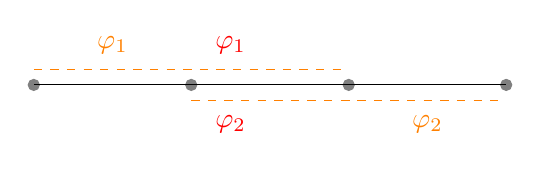
\begin{tikzpicture}
				%				[->,>=stealth',shorten >=1pt,auto,node distance=0,main node/.style={circle,draw}]
				%
					\filldraw [gray] (4,-1) circle (2pt)
				(2,-1) circle (2pt)
				%(0,0) circle (2pt)
				(0,-1) circle (2pt)
				%(0,-2) circle (2pt)
				%(6,0) circle (2pt)
				(6,-1) circle (2pt);
				%(6,-2) circle (2pt)	;
				%
				\draw [black]  (0,-1) -- (6,-1);
				%
				% \draw [black] (4,-1) -- (6,0);
				% \draw [black] (4,-1) -- (6,-2);
				% \draw [black] (0,0) -- (2,-1);
				% \draw [black] (0,-2) -- (2,-1);
				%
				\draw [dashed, orange] (0,-0.8) -> (2,-0.8) -> (4,-0.8);
				\draw [dashed, orange] (2,-1.2) -> (4,-1.2) -> (6,-1.2);
				
	%		{\tiny
				\node [orange] at (1,-0.5) {$\varphi_1$};	
				\node [red] at (2.5,-0.5) {$\hsAt\varphi_1$};
			\node [orange] at (5,-1.5) {$\varphi_2$};	
				\node [red] at (2.5,-1.5) {$\hsA \varphi_2$};
		%			\node (b0) at (4,-0.5) {$\rho'=\rho(0,i)\cdot \rho^{(j+1)]}$};	
		%			\node (a1) at (1.5,0.2) {$\rho(i)=$};
		%			\node (a2) at (2,0.2) {$\rho(j)$};
		%			\node (a3) at (1.65,0.5) {$Pattern(\rho,i)= Pattern(\rho,j)$};
		%			\node (a4) at (4.6,0.5) {$Pattern(\rho,k) =\{ p \in \Prop : \Ku,\rho^{k]} \models p\}$};
						
	%			}
				
			\end{tikzpicture}
\end{minipage}
%
    \caption{Trace-based semantic variant $\HS_\LinearTime$: neither past nor future are branching}
    \label{fig:LN}
\end{figure}

The state-based (see Figure~\ref{fig:ST}) and computation-tree-based (see Figure~\ref{fig:CT}) approaches rely on a \emph{branching}-time setting and differ in the nature of past. In the latter approach, past is \emph{linear}: each interval may have several possible futures, but only a unique past. Moreover, past is assumed to be \emph{finite} 
%(since program computations have a definite starting time) 
and \emph{cumulative}, that is, the story of the current situation increases with time, and is never forgotten. 
%
%Finally, the 
The trace-based approach relies on a \emph{linear}-time setting (see Figure~\ref{fig:LN}), where the infinite paths (computations) of the given Kripke structure are the main semantic entities. Branching is neither allowed in the past nor in the future.
%
Note that the linear-past (rather than branching) approach is more suited to the specification  of dynamic behaviors, because it considers states in a computation tree, while the branching-past approach considers machine states, where past is not very meaningful for the specification of behavioral constraints~\cite{LS95}.

The variant $\HS_\LinearPast$ is a natural candidate for an expressiveness comparison with the branching time logics  $\CTL$ and $\CTLStar$. The most interesting and technically involved result is the characterization of the expressive power of $\HS_\LinearPast$: $\HS_\LinearPast$ turns out to be expressively equivalent to finitary $\CTLStar$, that is, the variant of $\CTLStar$ with quantification over \emph{finite} paths. As for $\CTL$, a non comparability result can be stated.
%
%Conversely, 
The variant $\HS_\LinearTime$ is a natural candidate for an expressiveness comparison with $\LTL$: 
%As a matter of fact, 
we prove that $\HS_\LinearTime$ and $\LTL$ are equivalent (this result holds true even for a very small fragment of $\HS_\LinearTime$), but the former is at least exponentially more succinct than the latter. 

We complete the picture with a comparison of the three semantic variants $\HS_\stat$, $\HS_\LinearPast$, and $\HS_\LinearTime$. We show that, as expected, $\HS_\LinearTime$ is not comparable with either of the branching versions, $\HS_\LinearPast$ and $\HS_\stat$. The interesting result is that, on the other hand, $\HS_\LinearPast$ is strictly included in $\HS_\stat$: this supports $\HS_\stat$ as a reasonable and adequate semantic choice.

\begin{figure}[b]
%\vspace*{-0.4cm}
\centering
%\resizebox{\width}{\height}{%
\begin{tikzpicture}[-,>=stealth',shorten >=1pt,auto,semithick,main node/.style={rectangle,draw,inner sep=2pt}]  
%
\tikzstyle{gray node}=[fill=gray!30]
%
\node [main node](0) at (0,0) {$\HS_\LinearPast$};
\node [main node](1) at (0,1.5) {$\HS_\LinearTime$};
\node [main node](2) at (0,-1.5) {$\HS_\stat$};
\node [main node](3) at (2.5,0) {finitary $\CTLStar$};
\node [main node](4) at (2.5,1.5) {$\LTL$};
\node [main node](6) at (2.5,-1.5) {$\CTL$};
\node [main node](5) at (5,0) {$\CTLStar$};
%   
\draw [dashed] (0.east) to node {$\equiv$} (3);
\draw [dashed] (1.east) to node {$\equiv$} (4);
\draw [dashed] (3.east) to node {$<$} (5);
\draw [dashed] (0.north) to node [swap] {$\neq$} (1);
\draw [dashed] (0.south) to node {\rotatebox{-90}{$<$}} (2);
\draw [dashed] (2.east) to node [swap] {$\neq$} (6.west);
\draw [dashed] (2) [out=-40,in=270] to node [near end] {$\neq$} (5);
\draw [dashed] (0.south east) to node {$\neq$} (6.west);
\draw [dashed] (2) [out=135,in=225] to node {$\neq$} (1);
\end{tikzpicture}%}
\vspace*{-0.6cm}
\caption{Overview of the expressiveness results.}\label{results}
\end{figure}

The complete picture of the expressiveness results is reported in Figure~\ref{results}
(the symbols $\neq$, $\equiv$, and $<$ denote incomparability, equivalence, and strict %expressiveness 
inclusion, respectively).

\paragraph*{Organization of the chapter.}
\begin{itemize}
	\item In the next section we start with some preliminaries; in particular, in Section~\ref{sect:PTL} we recall the well-known PTLs $\LTL$, $\CTL$ and $\CTLStar$; in Section~\ref{sect:3sem} we define the three semantic variants of $\HS$ ($\HS_\stat$, $\HS_\LinearPast$ and $\HS_\LinearTime$). In Section~\ref{subs:vendingMach} we provide a detailed example which gives an intuitive account of the three semantic variants and highlights their differences.
	\item In the next three sections we analyze and compare the expressiveness of these logics.  
In Section~\ref{sec:CharacterizezionOfLeniarTimeHS} we show the expressive equivalence of $\LTL$ and $\HS_\LinearTime$. Then, in Section~\ref{sec:characterizationHSLinearPast} we prove the equivalence of $\HS_\LinearPast$ and finitary $\CTLStar$. In Section~\ref{sect:allSems} we compare the expressiveness of 
$\HS_\stat$, $\HS_\LinearPast$ and $\HS_\LinearTime$.
\end{itemize}
